\chapter{Compton camera application in nuclear medicine}\label{chap::5}


Most of the results presented in this chapter have been published in~\parencite{Fontana2017_PMB} and~\parencite{Fontana2017_APPB}.

\vfill

\minitoc

\newpage

\glsresetall
\glsunset{clarys} 

\section{Introduction}\label{chap5::sec::intro}

\gls{spect} is one of the most widespread techniques for nuclear medicine diagnostics examinations. In most of the clinical cases, a radiotracer is injected in the patient and the emitted $\gamma$-rays are collected by scintillating detectors coupled to physical collimation systems. This process leads to the reconstruction of a planar transmission image. Such a kind of imaging tool relies on the first idea proposed by Hal Anger~\parencite{Anger1958, Anger1964}, and it is now commercially available in different variants with peculiar features and applications. A complete system is often composed of at least two rotating detection heads, allowing a tomographic data acquisition and the reconstruction of a three-dimensional image of the radio-tracer distribution (see chapter~\ref{chap::1} for further details).

The main consequence of the collimation system is a forced trade-off between sensitivity and spatial resolution: The spatial resolution is completely determined by the collimator geometry, and it can only be increased by reducing the collimator hole size, at the expense of a reduction in the detector sensitivity since fewer photons survive the mechanical selection. Moreover, the collimator thickness and septa limit the primary energy acceptance, and the performance of Anger cameras generally downgrades as the energy increases.  

In order to overcome this mechanical collimator limitation, it is natural to move towards an \enquote{electronic collimation}, where the emitted photons are tracked and the emission point is reconstructed via Compton kinematics, and so to the application of Compton cameras in this field~\parencite{Everett1977, Singh1983}.

L. Han and colleagues~\parencite{Han2008} have performed a simulation work comparing a standard Anger camera and a Compton camera prototype for a fixed source energy of 364~keV (\gls{iod131} gamma ray emission). The expected enhanced detection efficiency associated to the Compton camera with respect to the Anger system was estimated to a factor 20 at the tested energy, while the spatial resolution was compared for equal imaging time. 

Starting from the results of Han and colleagues, we tested in simulation the performance of the \gls{clarys} Compton camera prototype (see chapter~\ref{chap::3}) for the application in \gls{spect}. The aim of this simulation work consists in extending the aforementioned study to a wide energy range, with simplified analysis methods. The \gls{clarys} prototype is compared to the Infinia Anger camera delivered by General Electrics Healthcare~\parencite{GeneralElectrics2006}. The detector performances are compared in terms of efficiency and spatial response with the exposure to mono-energetic point-like radioactive sources at different energies, ranging from 245~keV to 2.614~MeV. The noise components related to the target (patient), such as photon attenuation, photon diffusion, patient movements, are common for both detectors and not considered in this context.

It should be noticed that the Compton detection principle requires coincidences between the two detector sections (scatterer and absorber), so that the random coincidence rate plays a fundamental role in the complete system performance, like in \gls{pet} machines. The effect of these random coincidences will therefore be investigated. Moreover, a reliable Compton scattering cone reconstruction requires a precise energy resolution for the scatterer section of the detector. The influence of this parameter will be studied. Finally, the Doppler broadening effect will be quantified to give the physical limits of the Compton imaging technique knowing that silicon corresponds to the lowest $Z$ material available for gamma detection with precise energy resolution. A comparison with a different possible scatterer material is also performed for verification.

All the obtained results are discussed with direct reference to~\parencite{Han2008}, focusing on the possible advantages offered by the use of a Compton camera (in particular the \gls{clarys} prototype), which intrinsically introduce the possibility to update the clinical standards in terms of source kinds, energies and activities, examination duration, patient dose, imaging techniques.


\section{Material and methods}\label{chap5::sec::mat_met}
In this section, the sources of gamma rays simulated for the study are presented and discussed and the two simulated systems are described in detail, as well as the proposed analysis techniques. In addition to this, some comments are given about the criteria chosen to represent a relevant comparison between the two investigated detectors.

\subsection{Radioactive sources}\label{chap5::subsec::rad_sources}

Both  simulated systems have been exposed to monochromatic point-like gamma sources in air.
The performance of the two cameras has been studied in terms of spatial resolution and detection efficiency as a function of the gamma source energy, related to actual radioemitters, already used in clinical practice or suggested for this kind of application in previous works~\parencite{Nurdan2015}. The explored energy range was chosen having in mind the possible clinical usage of Compton systems like the one developed by the \gls{clarys} collaboration, to extend the present field of application of \gls{spect} imaging.

In \tablename~\ref{chap5::tab::table_sources}, the characteristics of the considered radioactive sources are given. Most of the sources do not emit gamma rays at a single energy, but only the ones selected for this study are presented in the table, together with the related branching ratio.

\begin{table}[!htbp]
\centering
\caption{Radioactive sources used in the comparison study. Decay mode list: EC for electron capture, $\mathrm{\beta}-$ for electron emission, $\mathrm{\beta}+$  for positron emission, IT for isomeric transition. Half-life expressed in days (d), hours (h) or minutes (m). Data extracted using the National Nuclear Data Center On-Line Data Service from the Evaluated Nuclear Structure Data File database, file revised as of (2017-05-17)~\parencite{Bath1992}.}
\label{chap5::tab::table_sources}
\begin{tabular}{m{3cm} P{3cm} P{3cm} P{2cm} P{2cm}}
\toprule
\rowcolor{myColorMainA!20}
\textbf{Isotope}           & \textbf{Gamma energy [keV]} & \textbf{Branching ratio [$\%$]}& \textbf{Decay mode} & \textbf{Half-life}  \\
\midrule
Indium 111 		  & 245 		&	94.1	      & EC          				 	& 2.8 d       \\
Iodine 131		  & 364		&	81.5      & $\mathrm{\beta}-$         	& 8 d         \\
Yttrium 91m		  & 555		&	95.0      & IT        				 	& 50 m        \\
Bismuth 212		  & 727		&	 6.7      & $\mathrm{\beta}-$         	& 60 m        \\
Iodine 132		  & 773		&	75.6      & $\mathrm{\beta}-$         	& 2.3 h       \\
Iron 59		  	  & 1099 - 1292 & 56.5 - 43.2	& $\mathrm{\beta}-$  	& 45 d     \\
Zinc 65		  	  & 1116 	&	50.0  	  & EC / $\mathrm{\beta}+$     	& 244 d       \\
Calcium 47		  & 1297		&	67.0      & $\mathrm{\beta}-$        	& 4.5 d       \\
Magnesium 28		  & 1342 	&	54.0 	  & $\mathrm{\beta}-$         	& 21 h        \\
Sodium 24		  & 1368		&	100.0        & $\mathrm{\beta}-$         & 25 h        \\
Potassium 42  	  & 1524		&	18.1        & $\mathrm{\beta}-$         	& 12 h        \\
Thallium 208		  & 2614		&	99.8        & $\mathrm{\beta}-$        	& 3 m      \\
\bottomrule

\end{tabular}
\end{table}

\subsection{Compton camera simulation and data analysis}\label{chap5::subsec::CC_simu}
\subsubsection{Simulation settings}\label{chap5::subsubsec::CC_settings}
\begin{figure}
  \centering
  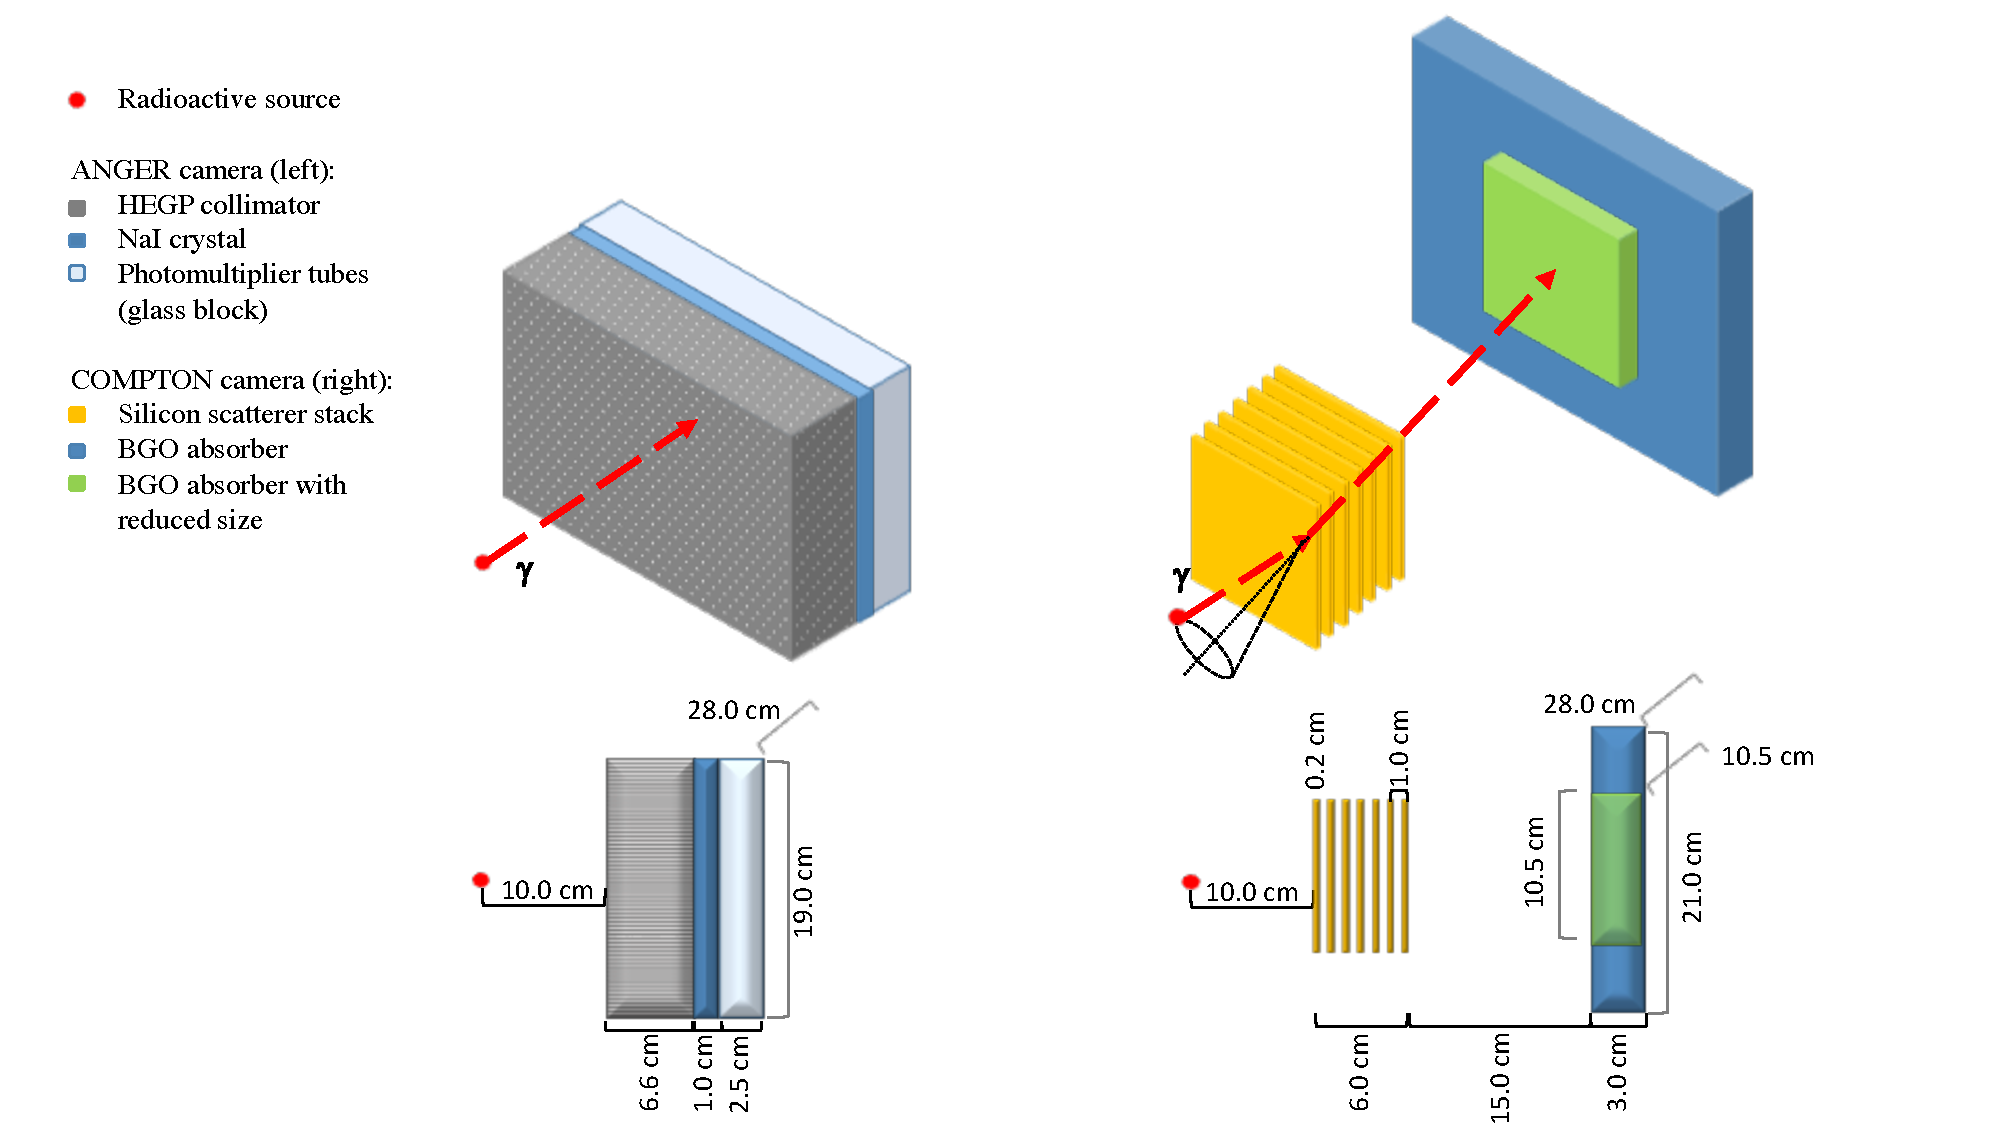
\includegraphics[width=1.1\linewidth]{03_GraphicFiles/chapter5_SPECTsimu/SPECT/schema_withRedAbs}
  \caption{Sketch of the simulated geometry of the two systems: Anger camera (left) and Compton camera (right), in 3 dimensions (top line) and side projection (bottom line).}
  \label{chap5::fig::geometry_schema}
\end{figure}

The simulation code for the Compton camera was developed with \gls{geant4} v.9.6 and the camera design is based on the specifications of the prototype at present under development by the \gls{clarys} collaboration, detailed in chapter~\ref{chap::3}. It should be noticed that the real size of the detector components slightly differs from the ones reproduced in simulation, which have been used in the code for simplicity. The geometric setting of the camera has initially been optimized for the application in ion therapy monitoring via prompt-gamma emission (see chapter~\ref{chap::4}) and has been adapted for \gls{spect} for this study in order to maximize the similarities between the two systems (Compton and Anger camera) in terms of detector acceptance, as detailed in the following. A \gls{spect} specific optimization would depend on the choice of the particular gamma energy and it has not been studied yet.

The distance between the last silicon plane (center) and the center of the absorber is set to 15~cm (see \figurename~\ref{chap5::fig::geometry_schema}).  Moreover, the absorber size has been adapted to be as close as possible to the Anger camera detector, maintaining the real \gls{bgo} block size. As a result, a matrix of 8$\times$6 blocks has been arranged, for a total surface of 28$\times$21~cm$^{2}$.
In the work of Han and colleagues~\parencite{Han2008} a Philips camera was described in GATE as Anger system and the same NaI absorber detector was adapted for the simulation of the Compton system with the introduction of silicon pad detectors as scatterer part. The two geometries compared in this study are slightly different but the common absorber size strategy has been maintained.

The values for energy and spatial resolution of the silicon and \gls{bgo} detectors used in the simulation were derived from the first tests performed on the detector prototypes (see chapter~\ref{chap::3}). For the silicon planes, the energy resolution is obtained from the \gls{enc}:

\begin{equation}
\sigma_{E}\, = \,W_{Si} \sqrt{\mathrm{ENC}^{2} + F_{Si}\frac{E_{dep}}{W_{Si}}},
\label{chap5::eq::E_res_ENC}
\end{equation}
where $F_{Si}\,=$0.115 is the silicon Fano factor, $E_{dep}$ is the energy released in the detector (in eV) and $W_{Si}$ is the energy required to create an electron-hole pair in silicon (3.6~eV). The \gls{enc} strongly affects the detector performance and it will be analyzed in the following. 

The spatial resolution was set according to the geometric parameters considering that the employed \glspl{dssd} have a total of 64 strips per side, with a pitch of 1.4~mm. The position of each interaction is set in the center of the strip where it is recorded in both detection planes. Charge sharing on neighbor strips can in principle allow for sub-pitch resolution, but according to preliminary characterization measurements the probability of such a kind of events is less than 10\%, and will be so neglected. The interaction depth is set as the center of the involved detector slab. The time resolution has been set to 20.0~ns \gls{fwhm} based on characterization measurements performed at the \gls{ganil} accelerator in France and in the lab at \gls{ipnl}~(see chapter~\ref{chap::3} and~\cite{Ley2015}).

The energy and timing resolution in the \gls{bgo} blocks are set to 21\% \gls{fwhm} and 3.0~ns \gls{fwhm} respectively, also based on characterization measurements performed with a cesium-137 source (662~keV gamma ray emission) and at the \gls{ganil} with prototype blocks. Concerning the spatial resolution, it has been verified that a sub-pixel resolution is not achievable on a single event basis, it is therefore fixed to the size of a single pixel (see chapter~\ref{chap::3}). Each block surface is streaked with an 8$\times$8 pixel matrix, 4.4~mm side, not reproduced in the simulation code. Each interaction is assigned to the center of the pixel where it is localized at the analysis stage, while the interaction depth is set at the center of the involved block.

\subsubsection{Data collection and analysis}\label{chap5::subsubsec::CC_analysis}
The radioactive source is placed at 10~cm distance from the first silicon detector, in the center of the scatterer stack transverse surface, and the number of simulated primaries is set to 10$^{7}$ gammas per energy step. To speed up the simulation, the primary gammas are emitted in a direction within the acceptance cone defined by the first Compton camera silicon plane. All results are then normalized to the full solid angle. 

All the events with at least one interaction in a silicon plane or at least one interaction in a \gls{bgo} block are stored during the simulation process in two data sets, one per detector section. A small fraction of events presents interactions in more than one scatterer plane ($<1$\% at 245~keV) and/or in more than one \gls{bgo} block ($\sim$8\% at 245~keV). This kind of events leads to ambiguities in the cone reconstruction, because the cone vertex and axis are not univocally defined, and it is not treatable via \gls{lm-mlem} reconstruction. Alternative reconstruction algorithms (such as the one included in the \gls{megalib}~\parencite{Zoglauer2006}) are able to estimate the most likely scenario for multiple interactions, at the expense of larger uncertainties and longer calculation time. The multiple interaction events, representing approximatly 8\% of the total at 245~keV, are then refused in this study for simplicity. This choice reduces the detection efficiency, so that the value obtained here could be seen as the lower limit for this kind of detection system. Once the two lists of events are built, the time coincidences are defined according to the source activity, the detector geometry and the single detection section time resolution. Finally, the emission points are reconstructed with a \gls{lm-mlem} algorithm developed by the \gls{creatis} institute in Lyon~\parencite{Lojacono2013}. The iterative algorithm reconstructs the Compton cones from the position and energy deposited in the scatterer stack and in the absorber blocks. A reconstruction volume must be defined, as well as a voxel 3 dimensional matrix in this volume. For this study the reconstruction volume has been fixed to $\mathrm{5\times5\times5}$~$\mathrm{cm^{3}}$ around the source, with a matrix of $\mathrm{51\times51\times51}$~voxels, and 15 algorithm iterations: this number is a compromise between reconstruction performance and calculation time.

\subsubsection{Compton camera study for SPECT application}\label{CC_SPECT}
As already mentioned in the introduction, a critical parameter in the Compton camera performances is the scatterer detector energy resolution. The goal of the instrumental development is to obtain an energy resolution as close to 1~keV ($\sigma_{E}$) as possible. The silicon detectors composing the stack have been tested at various temperatures in order to understand the behavior of the electronic noise and of the leakage current, and the read-out electronics is being developed with the aim to reduce the electronic noise (see chapter~\ref{chap::3}). The first laboratory tests showed an energy resolution at 25\textdegree{}C of approximately 10-15~keV \gls{fwhm} with a first read-out card prototype. The new card has been tested with simulated signals and gives a noise level closer to the expectations. No data are yet available to determine the detector energy resolution at different temperatures and with the final card version. In the simulation two different resolutions have been considered in order to verify the influence of this parameter on the final reconstructed image. The two chosen values are $\mathrm{\sigma_{E}\,=\,2\,keV}$ and $\mathrm{\sigma_{E}\,=\,4\,keV}$, corresponding to about 5~keV and 9.5~keV \gls{fwhm}, respectively, both calculated at 200~keV of released energy using equation~\ref{chap5::eq::E_res_ENC}. The influence of Doppler broadening has also been studied by disabling the Doppler effect in the simulation with the energy resolution set to $\mathrm{\sigma_{E}\,=\,2\,keV}$. Finally, a different possible scatterer material, \gls{cdte}, has been tested at the same resolution in order to verify the expected advantage given by the choice of silicon.

A coincidence study is mandatory to define the source activity to be used in the simulations dedicated to the benchmark with the Anger camera. Timing information is not included in the simulation code and a time structure must be assigned to the simulated primaries at the data analysis stage. A reference time is chosen randomly from an uniform distribution between 0~s and the data acquisition time and assigned to a primary photon. The data acquisition time ($\mathrm{T_{DAQ}}$) is calculated as the expected time needed for the emission of the desired number of primaries ($\mathrm{N_{primaries}}$) according to the source activity $\mathrm{A_{source}}$:

\begin{equation}
T_{DAQ}\, = \,\frac{N_{primaries}}{A_{source}}.
\label{chap5::eq::DAQ_time}
\end{equation} 

The source activity is not fixed at the simulation stage but only during data analysis afterwards. It can therefore be easily modified to perform a study of the camera performance with different kinds of sources. The scatterer and absorber interaction times are calculated with respect to the reference primary emission and included in the related data sets for the analysis.

Two sets of data are produced as output of this analysis, one for the scatterer and one for the absorber: Each element in the two sets corresponds to an interaction in the detector and includes the interaction 3 dimensional position, energy released, time with respect to the total data acquisition time and primary reference index provided by the simulation. The elements in the two data lists are ordered for increasing time. The detectors time resolution specified in section~\ref{chap5::subsec::CC_simu} and a time window set to 20~ns, corresponding to a 3~$\mathrm{\sigma}$ acceptance, are then used for the coincidence definition for different source activities. The time of each element in the absorber data set is compared to the time of the elements in the scatterer data set. A coincidence is defined when the scatterer event time is within the time window centered in the absorber event time. Each element is used one time only, and the analysis continues until the end of the absorber data list. If the two  elements (one from the scatterer data set and one from the absorber one) forming a coincidence have the same reference index, they correspond to interactions of the same primary photons and the coincidence is then a true one. If the reference index is different for the two elements, the coincidence is random. The number of true and random coincidences has been studied as a function of the source activity in a range of clinical interest between 1~MBq and 500~MBq, for a fixed energy value of 555~keV. The variation of the influence of random coincidences as a function of the energy was also investigated at a fixed source activity of 200~MBq.

The scatterer energy resolution and the source activity have been fixed for the benchmark study. The choice of their values is discussed in section~\ref{chap5::sec::Results_CC_SPECT}. 

Finally, with the same scatterer energy resolution and the source activity, the design of the Compton camera has been tested for this specific application, in particular for what concerns the number of employed scatterer planes. In addition to the original design configuration with seven \glspl{dssd}, additional sets of simulations have been performed at four reference primary gamma energy reducing the number of layers in each set, in order to assess the camera optimal configuration as a function of the gamma energy. The results are shown in section~\ref{chap5::subsec::Results_CC_SPECT_design} and are expressed according to the figures of merit used for the benchmark study (see section~\ref{chap5::subsec::fom}). 

\subsection{Anger camera simulation and data analysis}\label{chap5::subsec::Anger_descr}

\subsubsection{Simulation settings}\label{chap5::subsubsec::AC_settings}
The Anger camera system is simulated with \gls{gate} v.7.1 and it is based on the General Electrics Healthcare Infinia \gls{spect} system~\parencite{GeneralElectrics2006}, a commercial clinical camera with parallel hole collimator and \gls{naitl} scintillator. A single detection head is simulated in order to obtain a direct performance comparison to the Compton system.

The chosen configuration includes a \gls{hegp} lead collimator, 6.6~cm thick, with a surface of 28$\times$19~cm$^{2}$ (see \figurename~\ref{chap5::fig::geometry_schema}). The parallel hole grid is composed of hexagonal shaped holes, 0.2~cm radius, arranged in a quincunx structure, with a septal thickness of 1.8~mm. This collimator is optimized for energies below 364~keV, corresponding to the main gamma emission energy of \gls{iod131}. The \gls{naitl} crystal is simulated as a single block of 28$\times$19$\times$1~cm$^{3}$, in contact with the collimator back surface and read out by photo-multiplier tubes. The photo-multiplier grid is represented with a glass block of 2.5~cm thickness behind the crystal, with the same transverse surface (see \figurename~\ref{chap5::fig::geometry_schema}). The spatial and energy resolutions have been set according to the manufacturer specifications. Unless otherwise stated, their values correspond to one standard deviation. A lower detection energy threshold has been set to 80~keV.

The source is placed at 10~cm distance from the collimator surface (the distance chosen in the Infinia data sheet), as for the Compton camera with respect to the first silicon layer, and its transverse position corresponds to the center of the central collimator hole. For each source energy, 10$^{8}$ primary photons are simulated in 4$\pi$. An event corresponds to single or multiple interaction of a photon (or secondary particle produced by the photon interaction in the collimator) in the \gls{naitl} crystal. All the detected interactions are computed and the gamma interaction position is calculated during the simulation as the center of gravity of the positions of all the hits (energy transfers of secondary electrons), with the deposited energy as weight for the calculation. The deposited energy corresponds to the sum of the energies released during each hit. A set of interaction points and energy deposited is then stored. 

\subsubsection{Data analysis}\label{chap5::subsubsec::AC_dataTreat}
Four source primary energies have been chosen as references of the studied energy range and are used in the following to show the analysis method and the study results. The low energy range is represented by the \gls{ind111} emission at 245~keV, the first energy above the Anger camera construction limit has been set to 555~keV \gls{ytt91m}, while \gls{fe59} at 1099~keV and \gls{k42} at 1524~keV have been chosen to represent the medium and high energy range respectively. 

\figurename~\ref{chap5::fig::distr_with_fit} presents the raw radial event distributions for the four reference energies. Each distribution bin content is normalized according to the surface of the circular region corresponding to each radius. The first distribution bin always corresponds to the radius of the central collimator hole, with the partial inclusion of the surrounding septa. This choice is determined by the detector and collimator geometry and by the source position. It is possible to list three different kinds of events contributing to the radial distributions:
\begin{enumerate}
\item photons passing through the collimator holes without interactions,
\item photons traversing the collimator septa without interactions,
\item photons interacting in the collimator septa.
\end{enumerate} 
Only the first listed contribution transports true spatial information about the source location, and these photons generate the signal. All other kinds of events contribute to the background, which rapidly increases with the primary photon energy.

A background rejection is performed in order to extract the distribution corresponding to the signal. The complex background contribution cannot be determined analytically, we therefore approximated the background profile as a linear fit to the tail of the radial distribution. The fit limits have been defined as follows:
\begin{itemize}
\item[-] the lower limit is calculated as the radial distance where the photon flux on the \gls{naitl} detector is reduced to a fraction $\mathrm{\frac{1}{e}}$ by absorption effect in the collimator septa;
\item[-] the upper limit has been fixed to the half of the collimator smaller lateral side (95~mm), in order to avoid any kind of geometric effect due the binning choice or the normalization surface selection. The bin size creates artifacts in the radial distribution corresponding to the collimator limits, because three different geometries are involved: the circular surface covered by each distribution bin, the hexagonal shape of the collimator holes and the rectangular collimator geometry.
\end{itemize}
The estimated background profile is subtracted from the raw distribution and the result is used as reference of the image signal (\figurename~\ref{chap5::fig::distr_with_fit}).

\begin{figure}
\begin{subfigure}[b]{.5\textwidth}
  \centering
  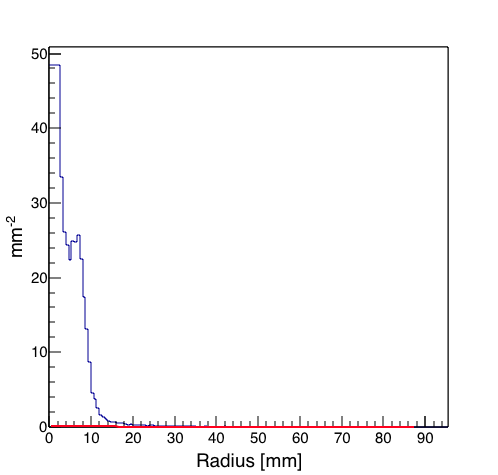
\includegraphics[width=.9\linewidth]{03_GraphicFiles/chapter5_SPECTsimu/SPECT/anger/radial_distr/fit_245keV}
  \caption{245~keV}
  \label{fig:rad_distr_fit_245keV}
\end{subfigure}
\begin{subfigure}[b]{.5\textwidth}
  \centering
  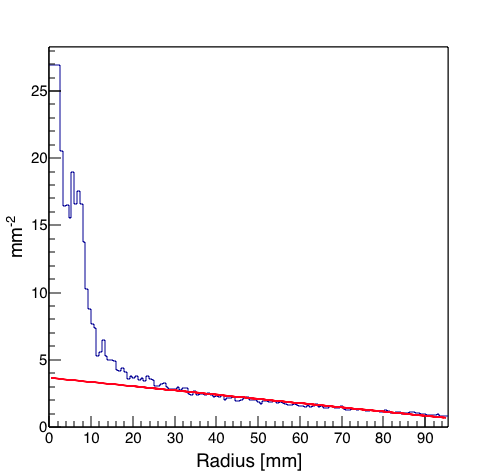
\includegraphics[width=.9\linewidth]{03_GraphicFiles/chapter5_SPECTsimu/SPECT/anger/radial_distr/fit_555keV}
  \caption{555~keV}
  \label{fig:rad_distr_fit_555keV}
\end{subfigure}
\begin{subfigure}[b]{.5\textwidth}
  \centering
  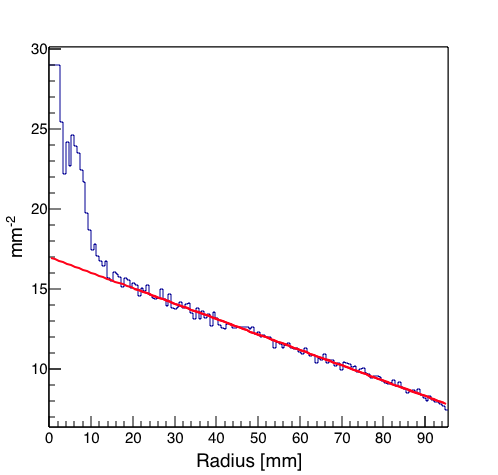
\includegraphics[width=.9\linewidth]{03_GraphicFiles/chapter5_SPECTsimu/SPECT/anger/radial_distr/fit_1099keV}
  \caption{1099~keV}
  \label{fig:rad_distr_fit_1099keV}
\end{subfigure}
\begin{subfigure}[b]{.5\textwidth}
  \centering
  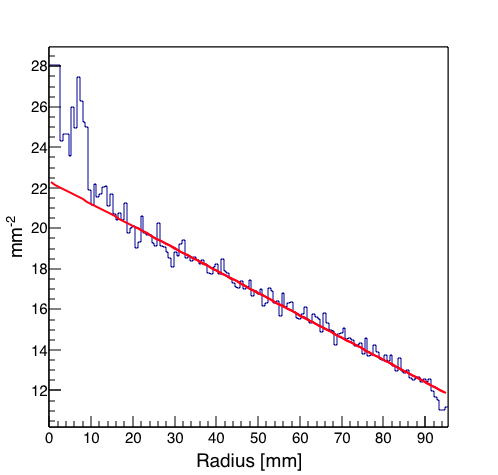
\includegraphics[width=.9\linewidth]{03_GraphicFiles/chapter5_SPECTsimu/SPECT/anger/radial_distr/fit_1524keV}
  \caption{1524~keV}
  \label{fig:rad_distr_fit_1524keV}
\end{subfigure}
\caption{Radial event distribution normalized by the circular surface corresponding to each bin for 4 representative source energies, with the linear fit performed for background rejection. The total number of simulated primaries for each data set is $\mathrm{10^{8}}$.}
\label{chap5::fig::distr_with_fit}
\end{figure}

Three validation tests have been performed in order to check this analysis method.\\ 
First, according to the geometry of the collimator and to the mass attenuation coefficient of \gls{naitl}~\parencite{Hubbell1987}, we evaluated the expected number of entries in the first distribution bin (before normalization), corresponding to the central collimator hole in front of the source. The calculation is performed with the attenuation law of photons in 1~cm of \gls{naitl}. A dedicated set of simulations has been performed equivalent to the ones for the Anger camera described in section~\ref{chap5::subsubsec::AC_settings}, but using an ideal detector and a reduced number of photons of 10$^7$. No uncertainties are applied on the position of photon interactions to avoid resolution effects and the background is estimated via a linear fit as described above. The obtained entries in the first distribution bin after the fit selection are compared to the ones obtained with the theoretical calculation. In \figurename~\ref{chap5::fig::firstBinCheck} the results are shown as a function of the source energy.


\begin{figure}[h]
  \centering
  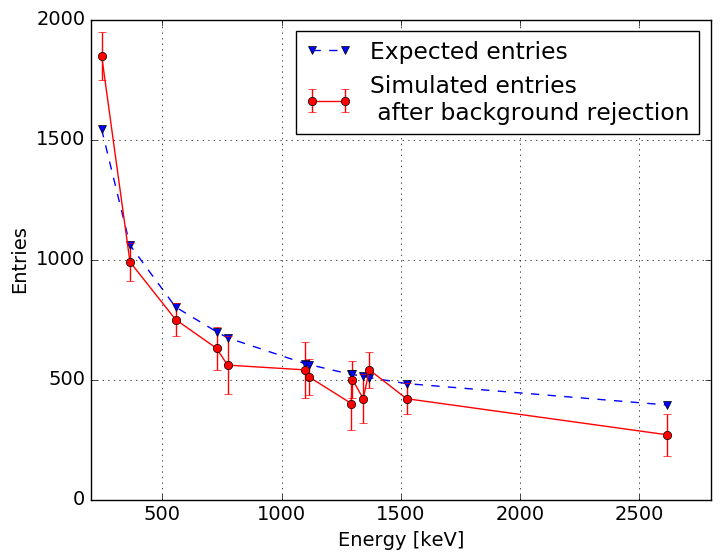
\includegraphics[width=.6\textwidth]{03_GraphicFiles/chapter5_SPECTsimu/SPECT/anger/firstBinInVSenergy}
\caption{Comparison between expected entries in the central collimator hole (blue dashed curve) calculated according to pure geometrical factors and detector interaction cross section and simulated detected entries after background rejection (red solid curve) with null spatial resolution (ideal detector) to avoid resolution effects and lower energy threshold set to 80~keV.}
\label{chap5::fig::firstBinCheck}
\end{figure}

There is a good agreement between the values calculated with the attenuation law and the simulation data selected with the fit-based background subtraction, and the detected variations from the ideal trend are within the statistical fluctuations. A slight overall effect of under-detection is observed (about 10\% on average), while the single value at 245~keV shows an opposite behavior (with a difference of less than 20\%). This is related to the chosen fit function.

As a second validation, an additional set of simulations has been performed with the same settings as defined in section \ref{chap5::subsubsec::AC_settings} but with an infinitely dense collimator. This configuration removes the background contribution given by the photons deflected via Compton interaction on the collimator septa. The raw radial distributions obtained with this set of simulation is compared to the radial distribution \enquote{derived} by the simulations with nominal settings after the application of the fit-based background subtraction. The results are shown in \figurename~\ref{chap5::fig::distr_infAbs}.

\begin{figure}
\begin{subfigure}{.5\textwidth}
  \centering
  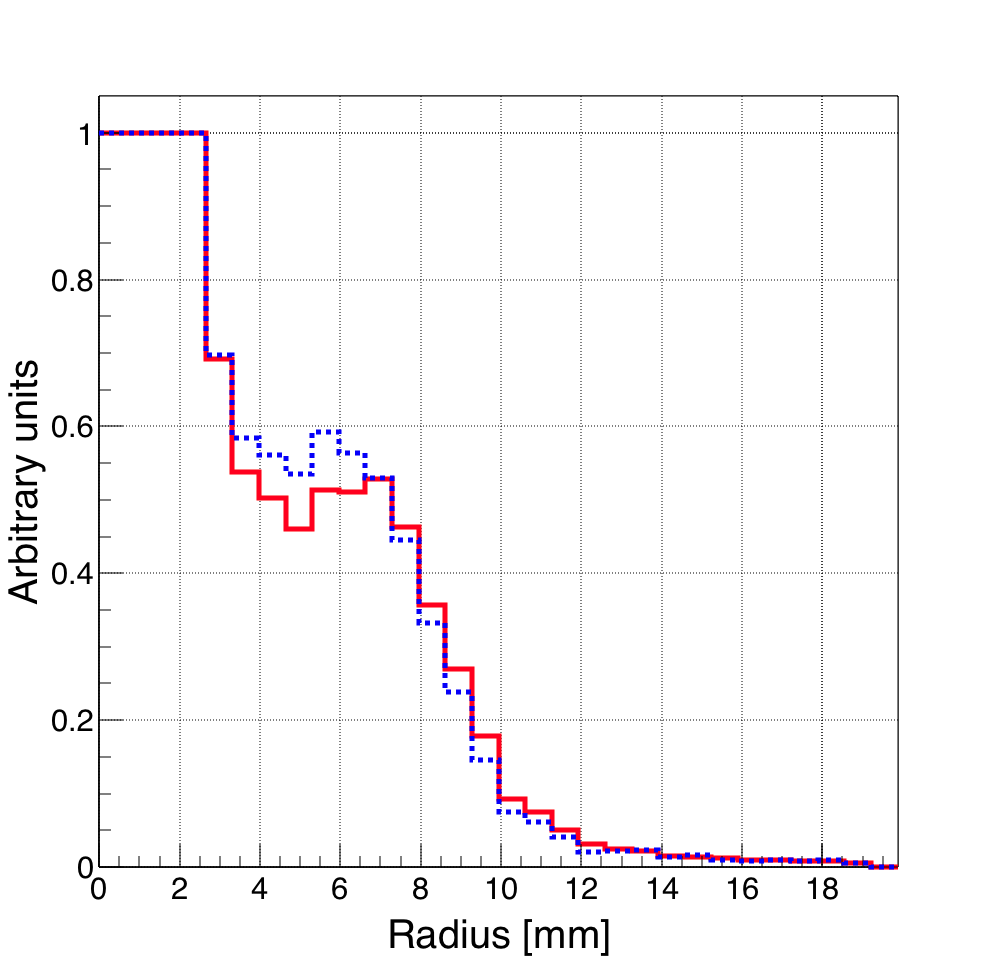
\includegraphics[width=.9\linewidth]{03_GraphicFiles/chapter5_SPECTsimu/SPECT/anger/inf_abs/overlap_infAbs_245keV_normMax}
  \caption{245~keV}
  \label{chap5::fig::rad_distr_infAbs_245keV}
\end{subfigure}
\begin{subfigure}{.5\textwidth}
  \centering
  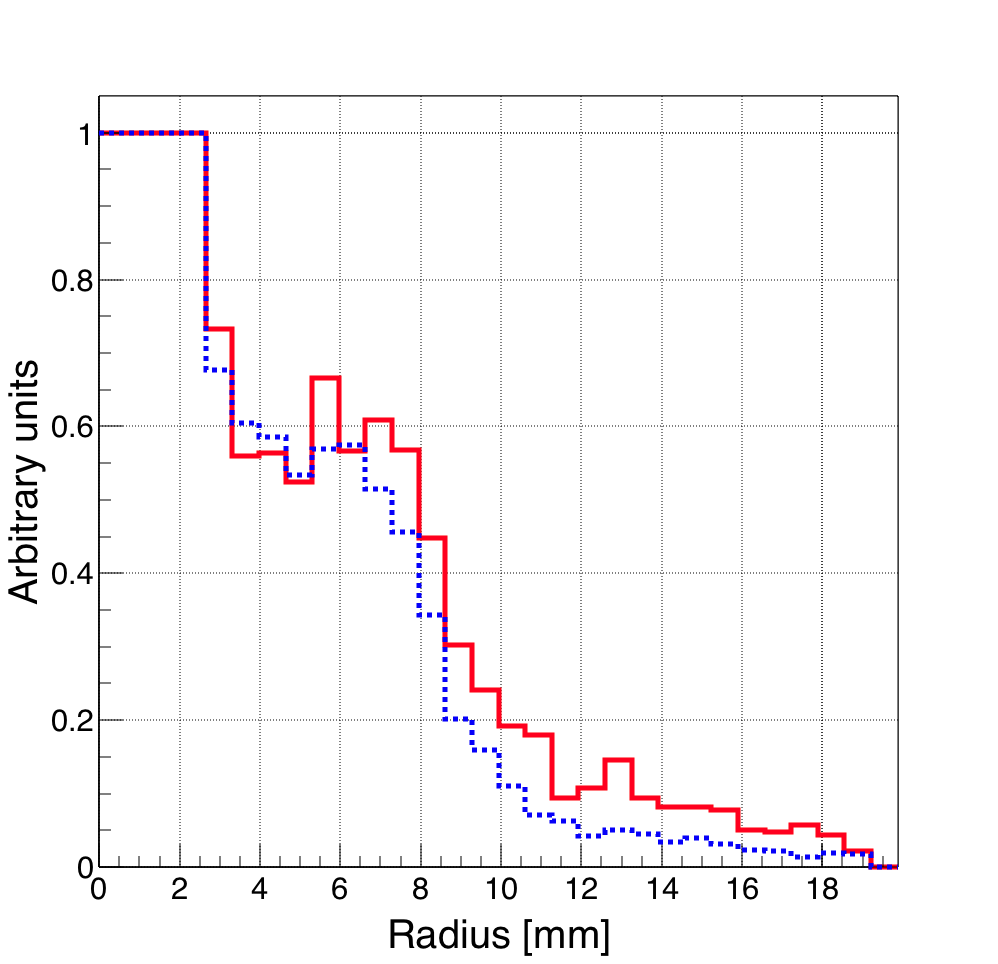
\includegraphics[width=.9\linewidth]{03_GraphicFiles/chapter5_SPECTsimu/SPECT/anger/inf_abs/overlap_infAbs_555keV_normMax}
  \caption{555~keV}
  \label{chap5::fig::rad_distr_infAbs_555keV}
\end{subfigure}
\begin{subfigure}{.5\textwidth}
  \centering
  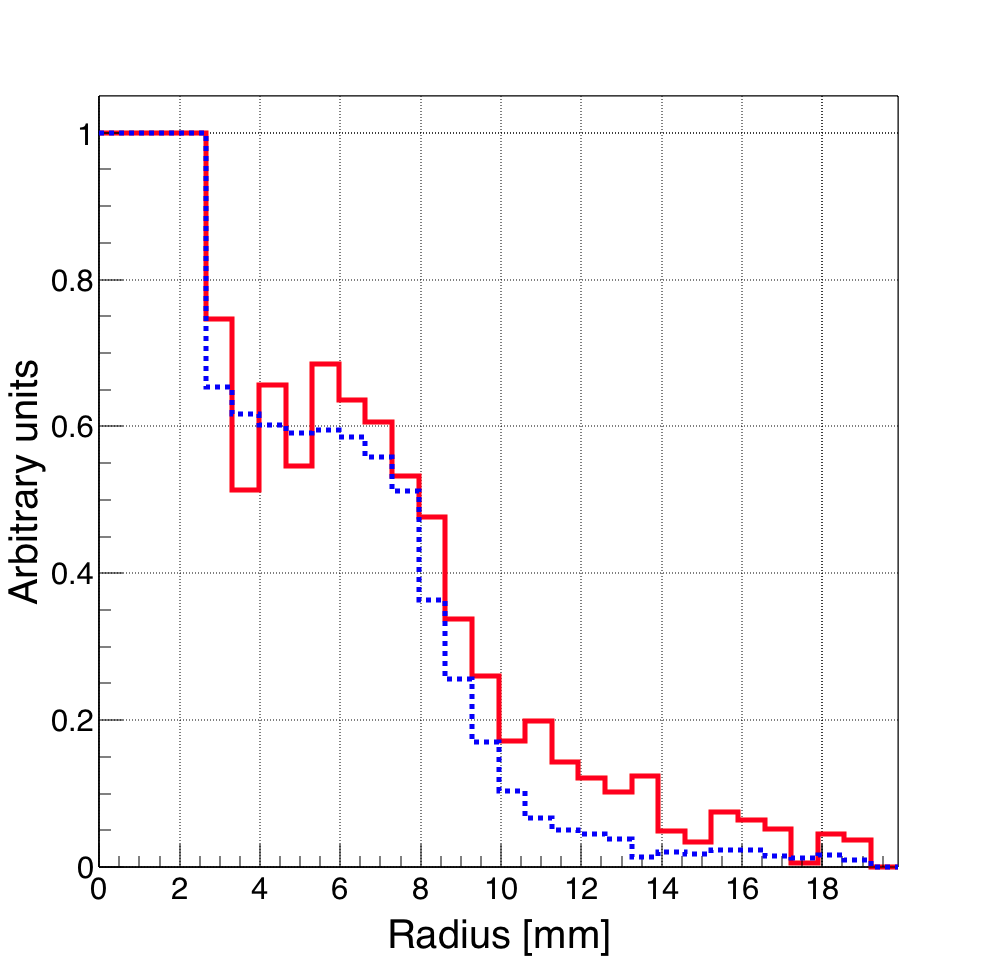
\includegraphics[width=.9\linewidth]{03_GraphicFiles/chapter5_SPECTsimu/SPECT/anger/inf_abs/overlap_infAbs_1099keV_normMax}
  \caption{1099~keV}
  \label{chap5::fig::rad_distr_infAbs_1099keV}
\end{subfigure}
\begin{subfigure}{.5\textwidth}
  \centering
  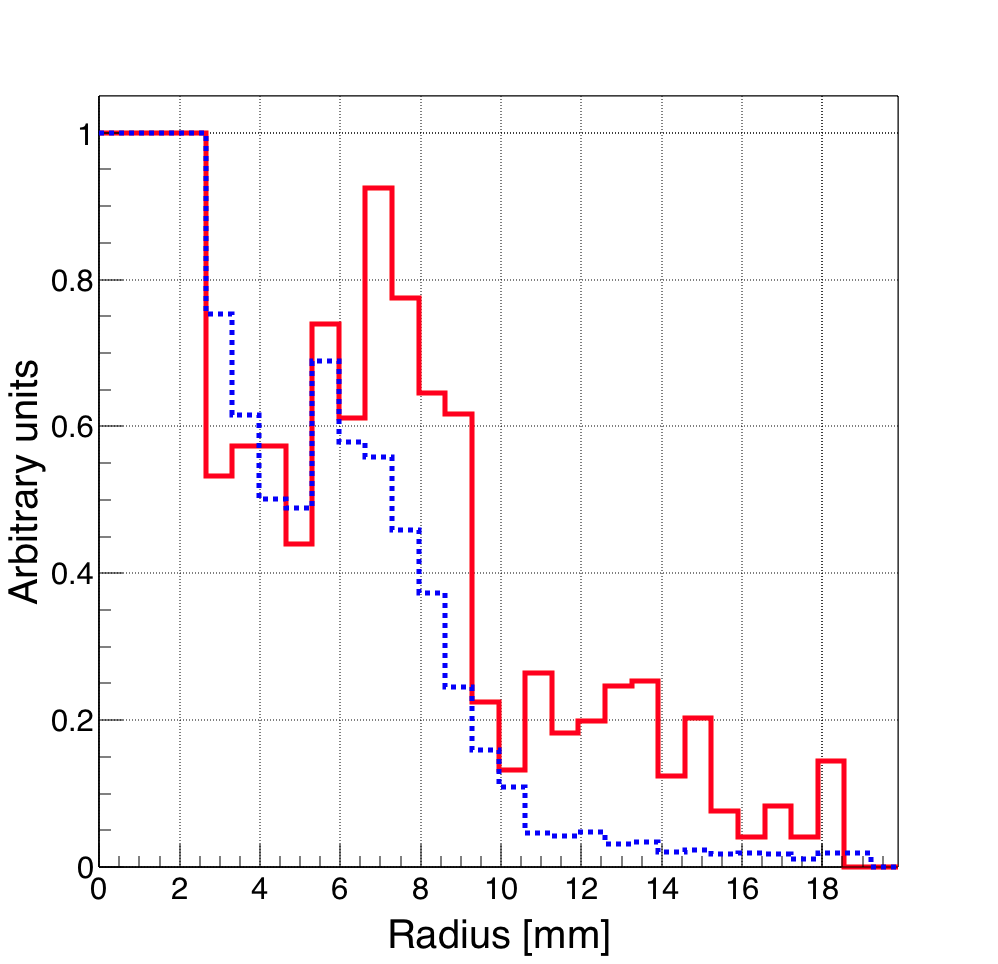
\includegraphics[width=.9\linewidth]{03_GraphicFiles/chapter5_SPECTsimu/SPECT/anger/inf_abs/overlap_infAbs_1524keV_normMax}
  \caption{1524~keV}
  \label{chap5::fig::rad_distr_infAbs_1524keV}
\end{subfigure}
\caption{Normalized radial distribution with background rejection (red solid lines) compared to normalized radial distribution for infinite density collimator (blue dashed lines).}
\label{chap5::fig::distr_infAbs}
\end{figure}

It can be noticed that the distribution overall trend is reproduced by the fit-based background rejection method, the main source of difference being probably the contribution of the scattering in the hole grid surrounding the central one.

The third validation test consisted in a set of simulation with a full lead collimator, with no holes. This configuration allows to estimate the distribution of events traversing the collimator with no interaction, with the aim of demonstrating the efficiency of the selection method to remove their contribution to the final image. \figurename~\ref{chap5::fig::distr_fullAbs} shows the comparison between the raw distributions (no event selection is applied) obtained with the standard configuration and with the full collimator. The amount of photons able to traverse the lead block at low energy (245 and 555~keV) is totally negligible, while at higher energies this kind of events creates an offset which follows the raw event distribution. Anyway, by observing the selection functions obtained by the linear fit in \figurename~\ref{chap5::fig::distr_with_fit}, the efficiency of the background employed rejection method in removing this contribution results clear.  

\begin{figure}
\begin{subfigure}{.5\textwidth}
  \centering
  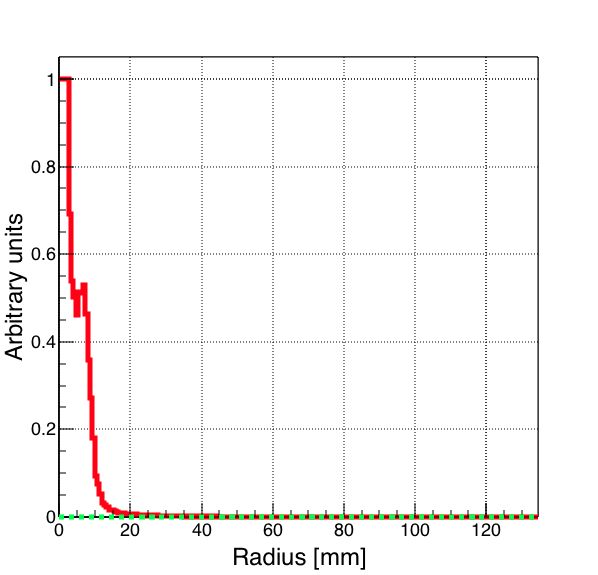
\includegraphics[width=.9\linewidth]{03_GraphicFiles/chapter5_SPECTsimu/SPECT/anger/no_holes/overlap_infAbs_245keV_normMax}
  \caption{245~keV}
  \label{chap5::fig::rad_distr_fullAbs_245keV}
\end{subfigure}
\begin{subfigure}{.5\textwidth}
  \centering
  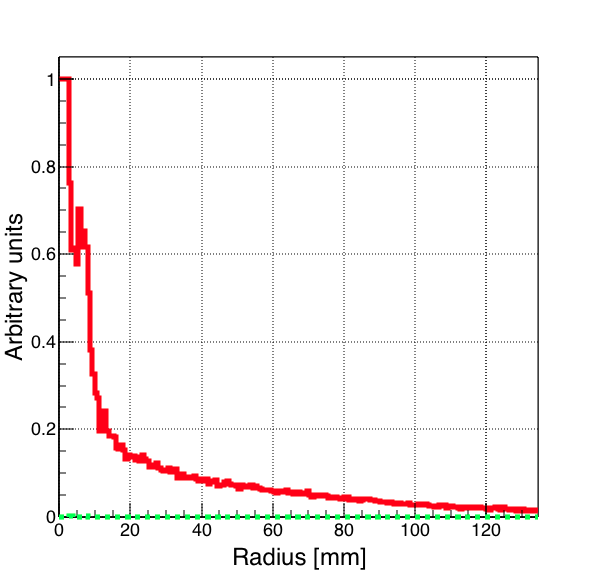
\includegraphics[width=.9\linewidth]{03_GraphicFiles/chapter5_SPECTsimu/SPECT/anger/no_holes/overlap_infAbs_555keV_normMax}
  \caption{555~keV}
  \label{chap5::fig::rad_distr_fullAbs_555keV}
\end{subfigure}
\begin{subfigure}{.5\textwidth}
  \centering
  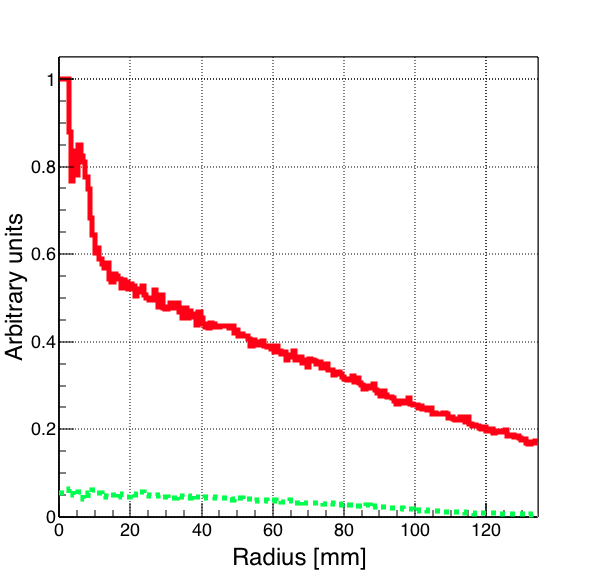
\includegraphics[width=.9\linewidth]{03_GraphicFiles/chapter5_SPECTsimu/SPECT/anger/no_holes/overlap_infAbs_1099keV_normMax}
  \caption{1099~keV}
  \label{chap5::fig::rad_distr_fullAbs_1099keV}
\end{subfigure}
\begin{subfigure}{.5\textwidth}
  \centering
  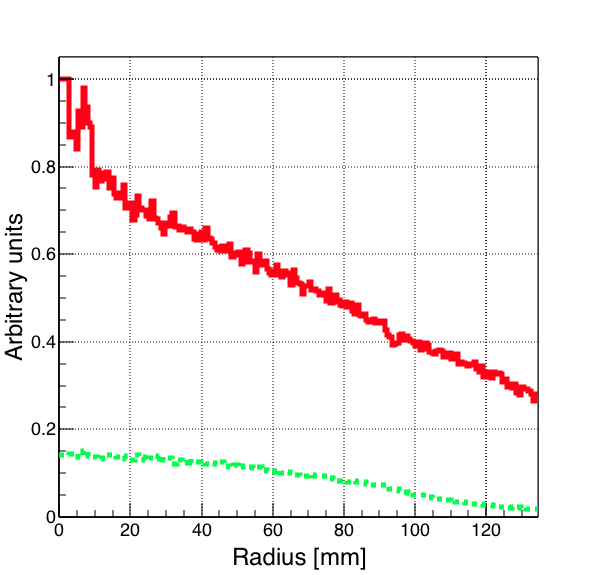
\includegraphics[width=.9\linewidth]{03_GraphicFiles/chapter5_SPECTsimu/SPECT/anger/no_holes/overlap_infAbs_1524keV_normMax}
  \caption{1524~keV}
  \label{chap5::fig::rad_distr_fullAbs_1524keV}
\end{subfigure}
\caption{Normalized radial distribution with no event selection (red solid lines) compared to normalized radial distribution for full collimator (green dashed lines). Both curves are normalized to the maximum of the raw radial distribution.}
\label{chap5::fig::distr_fullAbs}
\end{figure}

The linear fit appears to be a robust way to select the signal transporting spatial information from the source and is applied with no modification for the entire energy range, giving to the analysis method the desired consistency.

\subsection{Figures of merit for the comparison study}\label{chap5::subsec::fom}

The two cameras are studied and compared according to three figures of merit which refer to their main detection parameters: spatial resolution, detection efficiency, and signal-to-background ratio. The definition of these three values must be adapted to the two detectors, keeping in mind their differences: on one side the Anger camera provides a transmission image through a mechanical collimator, with no need for a reconstruction process and with a single detector component; on the other side, the Compton camera relies on event time-coincidences and needs a reconstruction algorithm to obtain the final spatial distribution.

In this study, the imaging process of a point source was simulated. The three figures of merit are therefore evaluated based on the radial event distribution, in order to profit of the radial symmetry of the simulated system.

For the Compton camera, the standard deviation of the radial distribution is used to express the detector spatial resolution, the detection efficiency is defined as the ratio between reconstructed events (via \gls{lm-mlem} algorithm) and total simulated primaries, and the signal-to-background ratio corresponds to the ratio between the number of reconstructed events and the total number of coincidences selected before the reconstruction with the coincidence analysis.

For the Anger camera, it is difficult to define the spatial resolution, as shown in~\parencite{Cecchin2015}. Here, we use the standard deviation of the signal radial distribution in order to be consistent with the Compton camera definition already proposed (the \enquote{signal} substantive means entries after background rejection). The detection efficiency is defined as the ratio between the number of signal events and the total number of simulated primaries. Finally, the signal-to-background ratio is evaluated as the ratio between the signal events (the entries in the radial distribution after the fit-based background rejection) and the total number of events recorded by the detector (the entries in the raw radial distribution).

\section{Results: Compton camera study for SPECT application}\label{chap5::sec::Results_CC_SPECT}
The results of the characterization of the \gls{clarys} Compton camera prototype for the application in \gls{spect} are presented in the following sections, dedicated to the study of the scatterer detector energy resolution and of the Doppler broadening effect, and to the analysis of the rate of random coincidences, respectively.

\subsection{Influence of Compton camera scatterer detector energy resolution}\label{chap5::subsec::Results_CC_SPECT_ENC}
\figurename~\ref{chap5::fig::ENC_study} shows the standard deviation of the radial distribution obtained after the \gls{lm-mlem} reconstruction (see section~\ref{chap5::subsubsec::CC_analysis}) as a function of the source energy for the two different analyzed noise levels (\gls{enc} = 500~e$^-$, corresponding to $\mathrm{\sigma_{E}\,=\,2\,keV}$, and \gls{enc} =1100~e$^-$, corresponding to $\mathrm{\sigma_{E}\,=\,4\,keV}$). The maximum detected difference is about 35\%, but the influence of the silicon detectors' energy resolution rapidly reduces at increasing energy. In the same figure, the results for the simulation without the Doppler broadening for the lowest energy resolution are shown. It is clear that this parameter has a strong influence for the Compton camera spatial resolution, at least for energies below 2.5~MeV. This result justifies the choice of silicon as scatterer material, because it is the lowest $Z$ available detector and therefore minimizes the Doppler contribution. This is underlined by the black curve corresponding to a \gls{cdte} detector, i.e. a higher $Z$ material than silicon. For this last study, the electronic noise level has been set for \gls{cdte} in order to have the same intrinsic resolution as for silicon ($\mathrm{\sigma_{E}\,=\,2\,keV}$ obtained with equation~\ref{chap5::eq::E_res_ENC}).

\begin{figure}
\begin{subfigure}[t]{.5\textwidth}
\centering
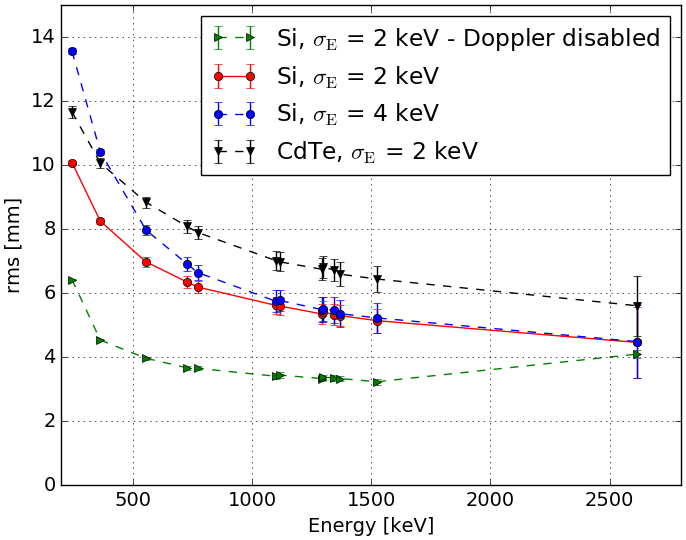
\includegraphics[width=\linewidth]{03_GraphicFiles/chapter5_SPECTsimu/SPECT/compton/ENC/rmsVSenergy_ENCstudy_Doppler} 
\caption{}
\label{chap5::subfig::ENCSi}
\end{subfigure}
\begin{subfigure}[t]{.5\textwidth}
\centering
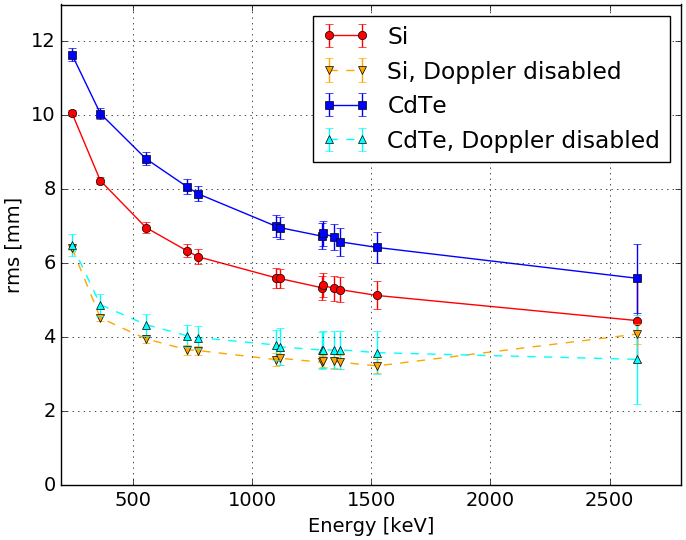
\includegraphics[width=\linewidth]{03_GraphicFiles/chapter5_SPECTsimu/SPECT/compton/ENC/rmsVSenergy_ENCstudy_Doppler_CdTe} 
\caption{}
\label{chap5::subfig::ENCSi}
\end{subfigure}
\caption{Reconstructed radial distribution standard deviation as a function of the source energy. Two energy resolution values are set to the silicon detectors ($\mathrm{\sigma_{E}\,=\,2\,keV}$ - red dots solid line - and $\mathrm{\sigma_{E}\,=\,4\,keV}$ - blue dots dashed line), the Doppler broadening effect has been removed (green horizontal triangles dashed line) and the scatterer material has been changed with \gls{cdte} solid state detectors (black vertical triangles dashed line), for a fixed energy resolution of $\mathrm{\sigma_{E}\,=\,2\,keV}$.}
\label{chap5::fig::ENC_study}
\end{figure}      
     
For the benchmark with the Anger camera, the \gls{enc} value of the Compton camera scatterer components has been fixed to 500~e$^-$, which corresponds to the expected average level of noise affecting the silicon detectors between -20\textdegree{}C (identified as the ideal working temperature) and 0\textdegree{}C (the silicon detectors are cooled down with a thermal-regulated box, see chapter~\ref{chap::3} for a detailed description) and with the final acquisition card (about 2~keV~$\sigma_{E}$). This value has to be experimentally verified.

\subsection{Compton camera coincidence study}\label{chap5::sec::Results_CC_SPECT_coinc}
\figurename~\ref{chap5::fig::timig_en_coinc}~(left) shows the numbers of true and random coincidences as a function of the source activity, ranging between 1 and 500~MBq in order to explore the whole range potentially employed in real examinations. The energy is set to 555~keV.  

\begin{figure}
\begin{subfigure}[t]{.5\textwidth}
\centering
  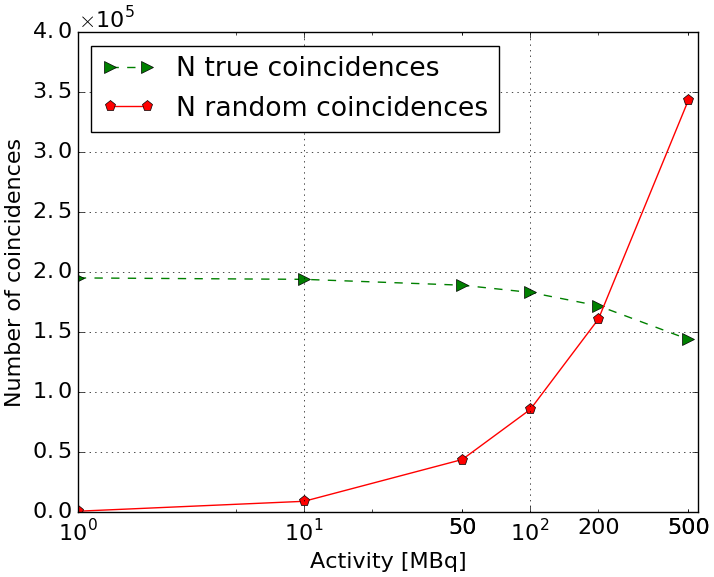
\includegraphics[width=.95\linewidth]{03_GraphicFiles/chapter5_SPECTsimu/SPECT/compton/timing/CoincidenceCounts}
  \caption{Number of coincidences \\ as a function of the source activity.}
  \label{chap5::fig::timing_counts}
\end{subfigure}
\begin{subfigure}[t]{.5\textwidth}
\centering
  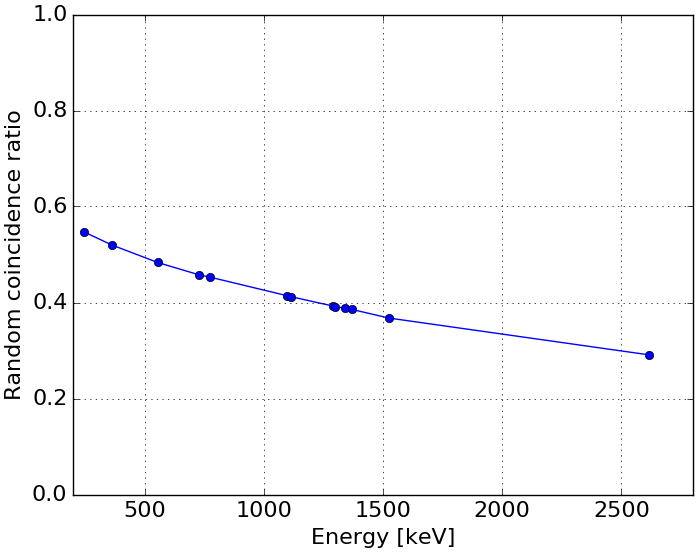
\includegraphics[width=.95\linewidth]{03_GraphicFiles/chapter5_SPECTsimu/SPECT/compton/timing/randomRatioVSenergy}
  \caption{Random coincidence ratio \\ as a function of the gamma energy.}
  \label{chap5::fig::timing_energy}
\end{subfigure}
\caption{(a): number of true (green) and random (red) coincidences as a function of the source activity in the range 1-500~MBq, for the reference energy of 555~keV. (b): Percentage of random coincidences as a function of the source energy, with a fixed source activity of 200~MBq. Compton camera parameters: time resolution \gls{fwhm} of 20~ns for silicon detectors, 3 ns for \gls{bgo} and a coincidence window of 40~ns. The source branching ratio has been set to 100\% for all sources for simplicity in the comparison of results.}
\label{chap5::fig::timig_en_coinc}
\end{figure} 

At 200~MBq source activity, the same amount of true and random coincidences is observed at 555~keV gamma energy. With activities above this value, the ratio between true and random coincidences is less than one. In principle the reconstruction \gls{lm-mlem} program can partially reject this kind of events and if we consider the expected important increase in detection efficiency guaranteed by the \enquote{electronic collimation}, it results clearly that it is not worth to employ high activity sources (or that a smaller camera can be considered at the expense of the examination time).

For the further analysis and the final detector comparison, the source activity has been then set to 200~MBq, and the number of random coincidences is studied as a function of the source energy. \figurename~\ref{chap5::fig::timig_en_coinc}~(right) shows the ratio of detected random coincidences over the total number of reconstructed coincidences (see Section~\ref{chap5::subsubsec::CC_analysis}) as a function of energy for a fixed activity of 200~MBq. The ratio decreases for increasing energies, because the product of independent interaction probabilities in two detectors decreases faster than the true coincidence one. Therefore, an increasing reconstruction efficiency with \gls{lm-mlem} is verified (see Section~\ref{chap5::sec::Results_benchmark}).

\subsection{Compton camera desing study}\label{chap5::subsec::Results_CC_SPECT_design}
The reconstructed events efficiency for four reference primary gamma energies is shown in figure~\ref{chap5::fig::design_eff} for five different scatterer configurations: starting from the original design with seven silicon layers, one layer has been removed for each simulation set, until a minimal scatterer stack composed of only three layers. \figurename~\ref{chap5::fig::design_rms} shows the results of the same sets of simulations for what concerns the reconstructed event radial distribution \gls{rms}.  

\begin{figure}[h!]
\begin{subfigure}[t]{0.5\textwidth}
\centering
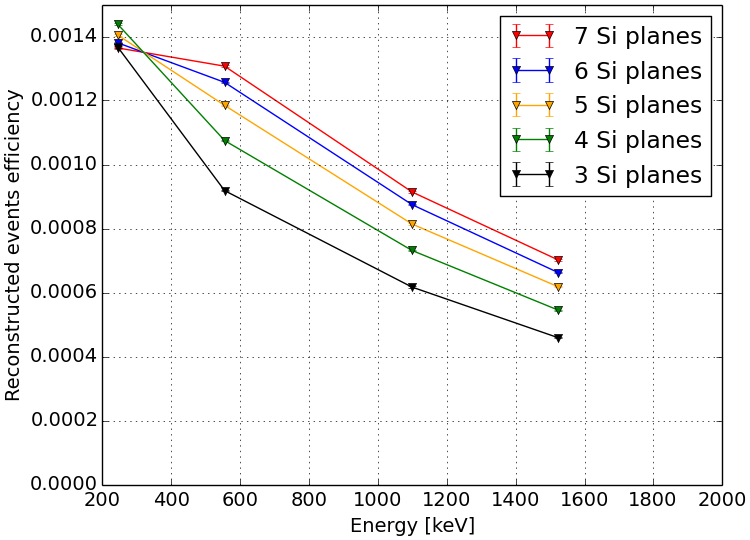
\includegraphics[scale=0.95]{03_GraphicFiles/chapter5_SPECTsimu/SPECT/compton/geometry/effVSenergy_NSiplanes.png}
\caption{Detection efficiency as a function of the source energy for five configurations of the scatterer stack: one layer has been removed for each simulation set. Source activity~=~200~MBq, Compton camera silicon detector $\mathrm{\sigma_{E}\,=\,2\,keV}$.}
\label{chap5::fig::design_eff}
\end{subfigure}  
\begin{subfigure}[t]{.5\textwidth}
\centering
  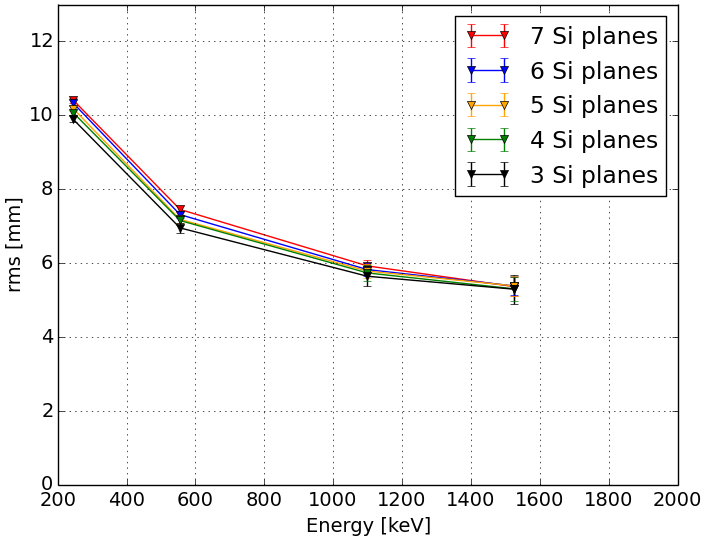
\includegraphics[width=.95\linewidth]{03_GraphicFiles/chapter5_SPECTsimu/SPECT/compton/geometry/rmsVSenergy_NSiplanes.png}
  \caption{Standard deviation of the radial event distributions as a function of the source energy for five configurations of the scatterer stack: one layer has been removed for each simulation set. Source activity~=~200~MBq, Compton camera silicon detector $\mathrm{\sigma_{E}\,=\,2\,keV}$.}
 \label{chap5::fig::design_rms}
\end{subfigure}
%\begin{subfigure}[t]{.5\textwidth}
%\centering
  %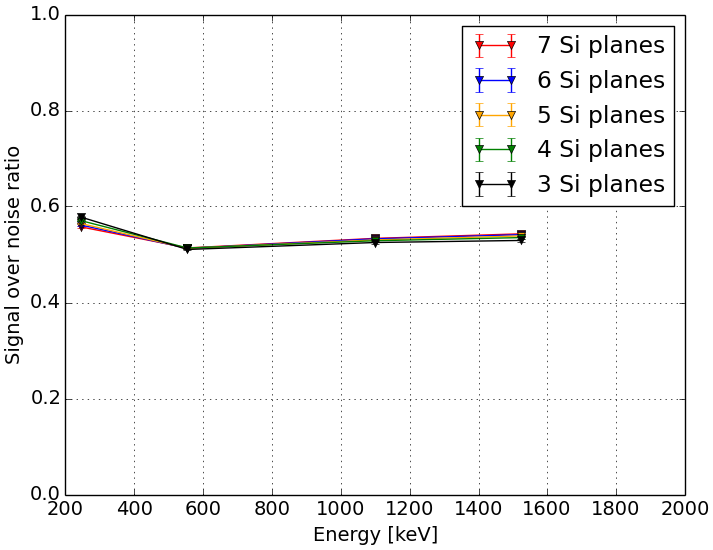
\includegraphics[width=.95\linewidth]{03_GraphicFiles/chapter5_SPECTsimu/SPECT/compton/geometry/ReffVSenergy_NSiplanes.png}
  %caption{Signal-to-background ratio as a function of the source energy for five configurations of the scatterer stack: one layer has been removed for each simulation set.. Source activity~=~200~MBq, Compton camera silicon detector $\mathrm{\sigma_{E}\,=\,2\,keV}$.}
  %\label{chap5::fig::design_SONR}
%\end{subfigure}
\caption{Results of the Compton camera design study: reconstructed events efficiency (left) and standard deviation of the radial event distribution (right) as a function of the primary gamma energies for four reference energies and five scatterer stack configurations, with seven, six, five, four and three layers.}
\label{chap5::fig::design}
\end{figure} 

Concerning the reconstructed events efficiency, an overall efficiency drop is observed for the scatterer configurations with more than four layers at 245~keV photon energy: this probably reveals an effect of total gamma absorption in the scatterer detector section, in parallel to an increased number of events deflected with large Compton angles which escape the absorber field of view. This effect is not confirmed at increasing gamma energy, already at 555~keV. In this energy range, the expected reduction of the overall efficiency for reduced number of scatterer layers (due to the diminished Compton effect probability) is verified. The radial distribution standard deviation shows minimal variations for the different tested configurations.\\
At very low gamma energy a scatterer configuration with four silicon scatterer planes appears to be the optimal solution. This is the energy range for which the Compton camera advantages with respect to the commercial Anger cameras are expected to be less remarkable, as explained and verified in the next sessions. At increasing energy, relevant to profit of the Compton camera advantageous features, the original \gls{clarys} camera design is verified to be the best configuration; this setup has been implemented for the benchmark study.   


\section{Results: Benchmark of Compton camera and Anger camera performance}\label{chap5::sec::Results_benchmark}

The analysis methods presented in section~\ref{chap5::subsubsec::CC_analysis} and section~\ref{chap5::subsubsec::AC_dataTreat} for the Compton and Anger camera, respectively, have been applied to the simulated data sets of the two cameras at all energies.

The radial distributions for Anger and Compton camera at the different reference source energies and a source activity of 200~MBq are shown in \figurename~\ref{chap5::fig::rad_distr_overlap}. The same reference energies selected in section~\ref{chap5::subsubsec::AC_dataTreat} are included here. The radial range is limited to the smaller collimator lateral size (95~mm), according to the fit limits imposed on the Anger camera data (see Section~\ref{chap5::subsubsec::AC_dataTreat}). The curves are normalized to 1 for an easier visual comparison.

\begin{figure}
\begin{subfigure}{.5\textwidth}
\centering
  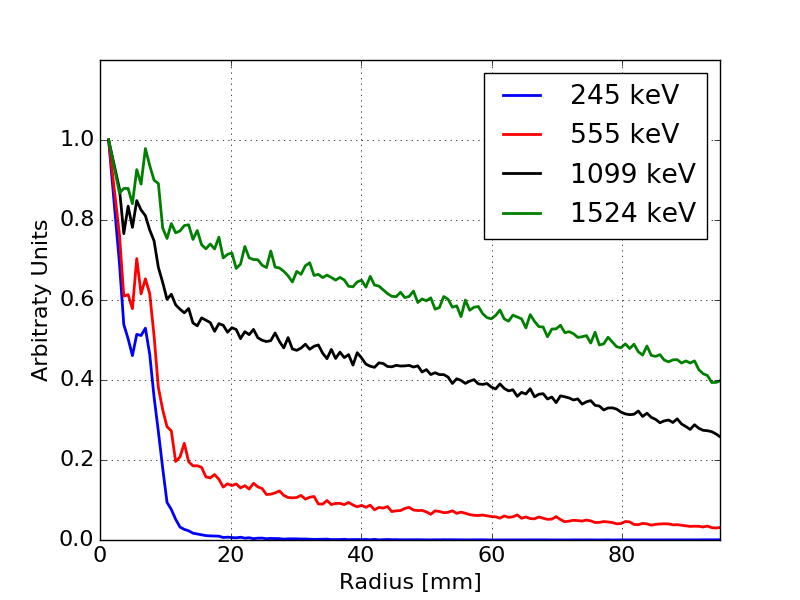
\includegraphics[width=\linewidth]{03_GraphicFiles/chapter5_SPECTsimu/SPECT/anger/radial_distribution_overlap}
  \caption{Anger camera events.}
  \label{chap5::fig::rad_distr_overlap_CA}
\end{subfigure}
\begin{subfigure}{.5\textwidth}
\centering
  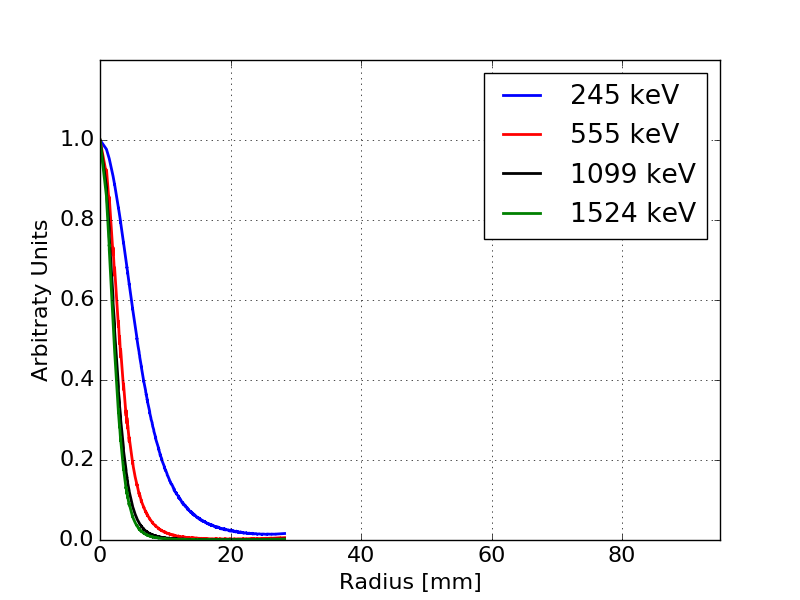
\includegraphics[width=\linewidth]{03_GraphicFiles/chapter5_SPECTsimu/SPECT/compton/radial_distribution_overlap_sel}
  \caption{Compton camera reconstructed events.}
  \label{chap5::fig::rad_distr_overlap_CC}
\end{subfigure}
\caption{Overlap of the normalized radial distributions for 4 selected source energies.}
\label{chap5::fig::rad_distr_overlap}
\end{figure} 
               
In Figures~\ref{chap5::fig::eff_energy_comp}, \ref{chap5::fig::RMS_energy_comp}, and \ref{chap5::fig::sel_eff_energy_comp}, the detection efficiency, the radial distribution standard deviation and the signal-over-noise ratio are respectively shown as a function of the source energy for the two sets of data. Uncertainties (one standard deviation) are reported for all the values and included in the data points when not visible.


\begin{figure}[h!]
\begin{center}
\hspace{0.4cm} 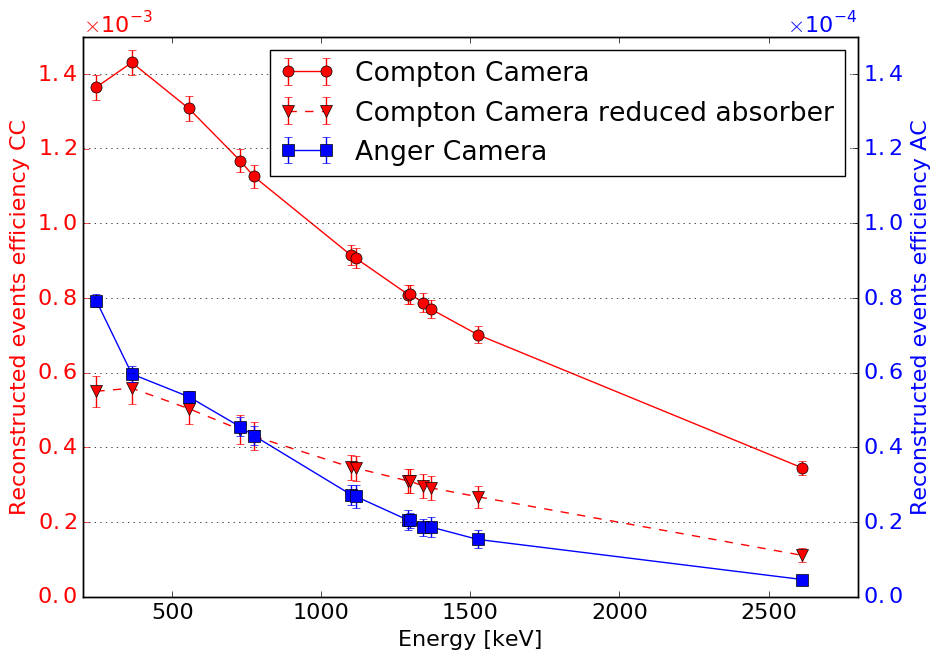
\includegraphics[scale=0.4]{03_GraphicFiles/chapter5_SPECTsimu/SPECT/comparison/reduced_absorber/effVSenergy_overlap}
\caption{Detection efficiency as a function of the source energy. Source activity~=~200~MBq, Compton camera silicon detector $\mathrm{\sigma_{E}\,=\,2\,keV}$.}
\label{chap5::fig::eff_energy_comp}
\end{center}
\end{figure}

\begin{figure}[h!]
\begin{center}
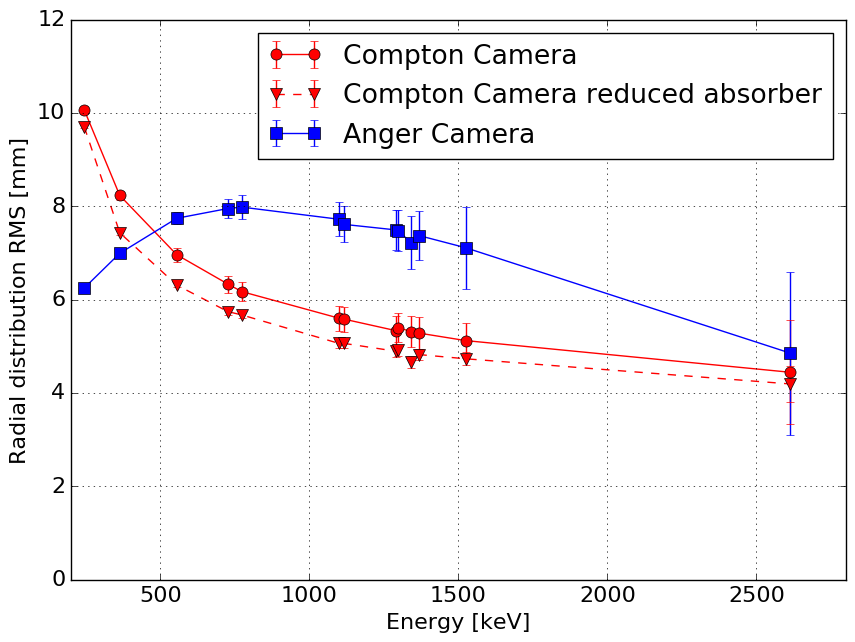
\includegraphics[scale=0.4]{03_GraphicFiles/chapter5_SPECTsimu/SPECT/comparison/reduced_absorber/RMSVSenergy_overlap}
\caption{Standard deviation of the radial event distributions as a function of the source energy. Source activity~=~200~MBq, Compton camera silicon detector $\mathrm{\sigma_{E}\,=\,2\,keV}$.}
\label{chap5::fig::RMS_energy_comp}
\end{center}
\end{figure}

\begin{figure}[h!]
\begin{center}
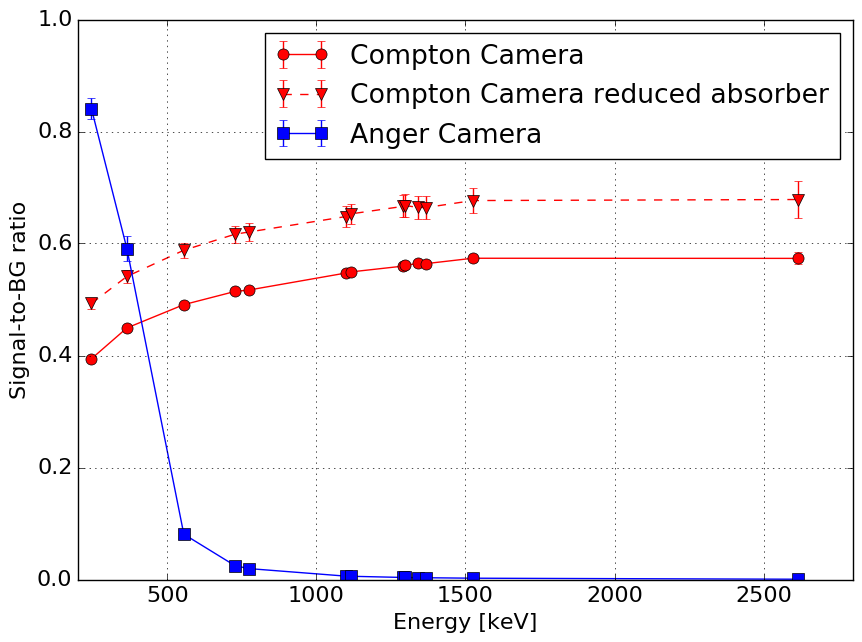
\includegraphics[scale=0.4]{03_GraphicFiles/chapter5_SPECTsimu/SPECT/comparison/reduced_absorber/SOBVSenergy_overlap}
\caption{Signal-to-background ratio as a function of the source energy. Source activity~=~200~MBq, Compton camera silicon detector $\mathrm{\sigma_{E}\,=\,2\,keV}$.}
\label{chap5::fig::sel_eff_energy_comp}
\end{center}
\end{figure}

From \figurename~\ref{chap5::fig::eff_energy_comp} one can point out the advantage provided by the absence of a physical collimation system in terms of detector efficiency. It should be noticed that two different scales are applied to \figurename~\ref{chap5::fig::eff_energy_comp} in order to show the two plots on the same figure and appreciate the variations with respect to the energy. The detection efficiency of the Compton camera is always more than a factor 20 higher than the one of the Anger camera. Although the images of the Anger and Compton cameras are based on different kinds of spatial information (a line and a cone, respectively), the Compton camera efficiency should allow a substantial reduction of the injected source activity and/or of the acquisition time. The efficiency of both cameras constantly decreases with increasing energy, because of the decreasing photon interaction probability. The only exception is found at the lowest considered energy of 245~keV in the Compton camera, due to an increased  probability of photon absorption in the scatterer and, in parallel, a larger fraction of events with wide Compton scattering angles at low gamma energy.

The standard deviation of the radial distribution, shown in \figurename~\ref{chap5::fig::RMS_energy_comp}, confirms the optimization of the chosen collimator for the Anger camera for low energies (below 364~keV). With the ad-hoc background subtraction operated here, which is not realistic for an extended source, the Anger camera outperforms the Compton one in terms of spatial resolution at low energies (by $>3$~mm at 245~keV and about 1.3~mm at 364~keV). However, above 500~keV, the Compton camera can provide a better spatial resolution with a difference ranging between a fraction of millimeter up to about 2~mm. For energies above 1.5~MeV, the two curves of standard deviation for the two cameras reach similar values ($<0.5$~mm difference at 2614~keV), but \figurename~\ref{chap5::fig::sel_eff_energy_comp} shows how the background rejection for the Anger camera and the MLEM reconstruction for the Compton system (see Sections~\ref{chap5::subsubsec::AC_dataTreat} and~\ref{chap5::subsubsec::CC_analysis}) affect this result. Above 364~keV, the selection for the background rejection of the Anger camera data drastically reduces the number of events contributing to the final image (the ratio between selected and detected events approaches zero). With an extreme selection, at very high energy the only events contributing to the final image are the events traversing the central hole of the collimator, resulting in an enhanced spatial resolution (see \figurename~\ref{chap5::fig::rad_distr_infAbs_1524keV}). The signal-to-background ratio of the Compton camera confirms the expectations concerning the reconstruction algorithm performance: if compared to \figurename~\ref{chap5::fig::timig_en_coinc}~(right), the curve in \figurename~\ref{chap5::fig::sel_eff_energy_comp} shows how the rejected events correspond approximately to the amount of random coincidences.
              

\section{Summary and discussion}\label{chap5::sec::Conclusions}

The Compton camera under development by the \gls{clarys} collaboration is now at the characterization stage. Originally designed and optimized for the application in ion beam therapy monitoring  for the detection of prompt-gamma rays in a wide energy range (between some hundreds of keV until about 10~MeV), it is here studied as \gls{spect} detector in comparison to a commercial system based on the Anger gamma camera design.

The expected significant enhancement in terms of detection efficiency, for comparable imaging performance in terms of spatial accuracy, has been already proven in simulation in~\parencite{Han2008} with a silicon-sodium iodide based Compton camera prototype at a single primary energy of 364~keV. A factor 20 efficiency gain has been reported.

First of all, the present simulation study aimed to extend these results by testing the two detectors at increasing primary gamma energies, ranging from 245~keV to 2614~keV. A common analysis method has been defined in order to obtain comparable results, always keeping as reference the final image. The results were directly compared in terms of  detection efficiency, spatial resolution (standard deviation of the radial event distribution) and event selection (background rejection for the Anger camera and \gls{lm-mlem} algorithm selection for the Compton camera) via the definition of three figures of merit.

A preliminary study has been performed on the simulated Compton camera data in order to fix the main parameters of the camera simulations, namely the energy resolution of the silicon scatterer detectors and the source activity determining the coincidence rate. Two \gls{enc} values have been studied, resulting in a maximum difference in spatial resolution of 35\% at the lowest energies, rapidly decreasing at increasing primary energy. A value of \gls{enc} = 500~e$^-$ has been chosen as the closest to the instrumental development expectations and first tests. The influence of the Doppler broadening on the spatial resolution has been also estimated in a factor $\sim$1/3 at 500 keV, then reduced up to $\sim$0 at 2.5 MeV of primary gamma energy, with fixed energy resolution ($\mathrm{\sigma_{E}\,=\,2\,keV}$ - \gls{enc} = 500~e$^-$) in the silicon detectors. Moving to the coincidence rate analysis, at the reference energy of 555~keV and with detector time resolution set according to first characterization results, the simulated data have been analyzed by reproducing a source activity in the range 1-500~MBq. The result shows the expected increase in the random coincidence rate at increasing source activity, with a ratio between true and random coincidences close to one at 200~MBq. This value has been chosen as clinical reference for the comparison analysis. In addition to this, the geometrical configuration of the scatterer stack has been studied in order to check alternative setups with reduced number of \glspl{dssd}; this study confirmed the choice of seven planes, implemented for the benchmark analysis. 

The results discussed in section~\ref{chap5::sec::Results_benchmark} confirm the conclusion of Han et al. about the advantage given by the usage of a Compton system and show how the gain factor in the detector efficiency is maintained at increasing energy. Concerning the detector spatial resolution, the Compton camera outperforms the Anger system at energies above about 500~keV. The Anger camera spatial resolution can be boosted by aggressive background subtraction in the considered case (point-like source image), at the expense of a drastic signal suppression. However, this approach is not reproducible and exploitable in actual clinical conditions and the obtained results are not comparable to the Compton camera performance at the same energy.

The results of this work clearly show the potential of the Compton camera for the application in nuclear medicine examination, opening new possibilities for the clinical implementation. The studied detector has originally been designed and optimized for another application, and it has only been adapted for \gls{spect} here, but not yet optimized in terms of detector geometry (size, position, and inter-detector distances). For an optimized detector, performance is therefore expected to be improved with respect to the presented results. In future development, the reconstruction \gls{lm-mlem} algorithm should be adapted to this application and the reconstruction parameters should be studied to further enhance the final performance, in particular for what concerns random coincidence rejection.

Anyway, these first evidences already allow one to investigate the possible modifications introduced by the clinical set of Compton detection systems. The enhanced detection efficiency in parallel with comparable spatial performances paves the way to the diffused usage of less active sources, or alternatively allows a substantial reduction of examination time: as a result, the dose delivered to the patient would be reduced. On the other side, the possible introduction of sources with higher primary emission energy will reduce the effect of photon attenuation in the patient (not studied in this simulation work), improving by definition the spatial information and further reducing the effective dose delivered to the patient. Simple analytic calculations can show how a photon attenuation of about 66\% is foreseen for 364~keV photons in 10~cm of water, while the effect is reduced, for example, to 49 \% at photon energy of 1099~keV~\parencite{Hubbell1987}. Higher energies can be employed also with Anger cameras, at the expense of introducing thicker collimators with reduced holes size, with the result of a reduced efficiency with respect to the analyzed \gls{hegp} collimator.
Furthermore, a possible implementation of Compton cameras is also foreseen for targeted radionuclide therapy, where the radionuclides used in clinics often have gamma radiation emission at relatively high energy. This signal is difficult to be detected and treated with conventional \gls{spect} cameras, while the Compton detection technique could make it quantitatively exploitable in clinical practice, for both pre- and per- treatment images.
   
Even though Compton cameras intrinsically lead to 3 dimensional images with a single detector head, the spatial resolution associated to the direction normal to the detector planes has to be more deeply studied, but this feature is an additional point in favor of the introduction of Compton systems in the clinical environment, moving beyond the tomographic concept and towards more compact detector solutions. Several studies are ongoing in order to improve the image reconstruction algorithms and, so, the 3 dimensional imaging performance~\parencite{Kuchment2016}. Different detection approaches can also, in principle, lead to improved image quality in 3 dimensions, such as the Compton electron tracking~\parencite{Sonoda2015, Kabuki2007}. Moreover, a further enhancement in image reconstruction should be given by the measurement of the photon depth of interaction: the photon is assumed to interact in the center of the detector components for our prototype, while perpendicularly segmented detectors can ensure an improved resolution in the third dimension and a resulting enhanced reconstruction accuracy, also involving better 3 dimensional imaging capabilities. 

The advantages of the Compton detection principle are here shown thanks to a first detector prototype, but there is still wide room for improvement.       

Once the \gls{clarys} Compton camera will be completed and characterized, tests in clinical environment are foreseen in the field of medical imaging. The actual potential of such a kind of detector will be then quantified with experimental data.

\clearpage
%\printbibliography[heading=subbibintoc]
